\chapter{Blide}

\textsf{
In questo capitolo viene presentato \emph{Blide} (Blite Integrated Development
Environment) un tool che racchiude un ambiente di esecuzione locale e
fornisce un interfaccia grafica che permette di svolgere in maniera integrata
tutte le operazioni legate allo sviluppo di programmi Blite. 
% Nella prima parte
% del capitolo vengono descritte le caratteristiche e le funzionalità
% dell'interfaccia, mentre nella seconda parte se ne presetano alcuni
% esempi di utilizzo.
In questo capitolo vengono descritte le caratteristiche e le funzionalità
dell'interfaccia.
}

\section{Un IDE per Blite}

Per verificare se uno strumento è funzionale, la cosa migliore da fare
è provarlo. In tal senso per verificare se il linguaggio e il motore di
esecuzione realizzati risultino veramente utilizzabili è stato sviluppato un
vero e proprio IDE che permetta di scrivere rapidamente e testare, tramite
l'esecuzione di simulazioni, i programmi Blite.

% Oltre al motore di esecuzione si è realizzato un vero e proprio IDE per
% sviluppare i programmi Blite. 
Questo strumento prevede la possibilità di
gestire i file con le definizioni dei processi, editarli, compilarli e metterli
in esecuzione. E' presente anche la funzionalità per visualizzare, tramite una
rappresentazione grafica, l'esecuzione delle istanze di processo.

Blide è stato realizzato tramite la piattaforma \emph{NetBeans Platform}
[NBPlatSite], un framework studiato per facilitare lo sviluppo di applicazioni
Java con interfaccia grafica. E' stato scelto tale progetto per la sua
completezza e per il modello architetturale offerto. 

NetBeans Platform permette allo sviluppatore di realizzare le proprie
applicazioni componendo diversi moduli, ciascuno dei quali offre una
funzionalità specifica. La modularizzazione molto fine e la gestione
formale delle dipendenze permettono di costruire applicazioni riuscendo a
selezionare in modo molto mirato solamente i moduli realmente necessari e
quindi a mantenere limitate le dimensioni complessive dell'applicazione. 
Per una presentazione approfondita a NetBeans Platform si consulti
[RichClientApp].

\begin{figure}[t!]
\begin{center}
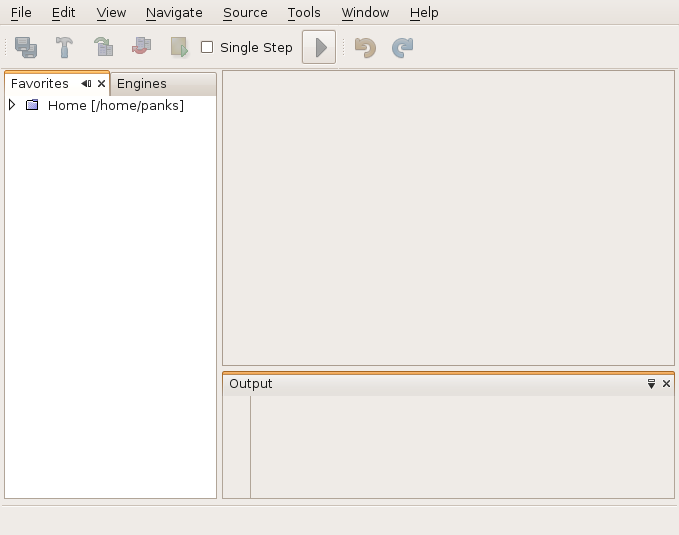
\includegraphics[scale=0.60]
{blide/dia/Blide1}
\caption[Blide Schermata]{Come si presenta Blide al primo avvio.}
  \label{fig:blide1}
\end{center}
\end{figure}
 
In Figura \ref{fig:blide1} è presentata l'interfaccia di Blide al primo avvio. 
Oltre alle consuete barre dei menù e dei pulsanti posizionate in alto
l'applicazione presenta quatro aree distinte

\begin{enumerate}
  \item Un pannello identificato dall'etichetta \emph{``Favorites''} che
  permette di accedere al filesystem e organizzare i file ``preferiti''
  in raggruppamenti logici.
  \item Un pannello identificato con l'etichetta \emph{``Engines''} in cui è
  possibile accedere ai motori di esecuzione attualmente disponibili, alle
  definizioni di processo e alle istanze create da queste.
  \item Un'area centrale in cui verrano visualizzati gli editor con i file
  sorgenti e le rappresentazioni grafiche delle istanze eseguite.
  \item Un pannello in basso in cui è possibile visualizzare l'output di
  sistema, come per esempio l'esito della compilazione dei programmi Blite.
\end{enumerate}

Di seguito andiamo ad analizzare più nel dettaglio queste aree e altre
funzionalità dell'interfaccia di Blide.

\subsubsection*{Favorites - Gestione dei Sorgenti Blite}

Abbiamo detto che questa area permette di accedere al filesystem, in realtà
non offre un'unica visione dell'albero come i consueti file manager, ma
permette in pratica di visualizzare direttamente più sotto alberi del
filesystem. Di fatto l'utente può selezionare un direcotry e con la funzione \emph{``Add to
Favoritess\ldots''} aggiungere tale directory, con tutto il suo sotto albero,
come una nuova radice che compare direttamente nel pannello. In questo modo l'utente
si può creare una specie di \emph{Bookmarks} alle directory a cui accede
maggiormente e in cui probabilmente ha salvato i file di lavoro. Da notare che
tali configurazioni vengono salvate automaticamente dall'applicazione e al
successivo riavvio l'utente si troverà mantenute le scorciatoie alle directory
preferite. Al primo avvio l'applicazione mostrerà come unica risorsa favorita
la directory ``home'' dell'utente.

\begin{figure}[h]
\begin{center}
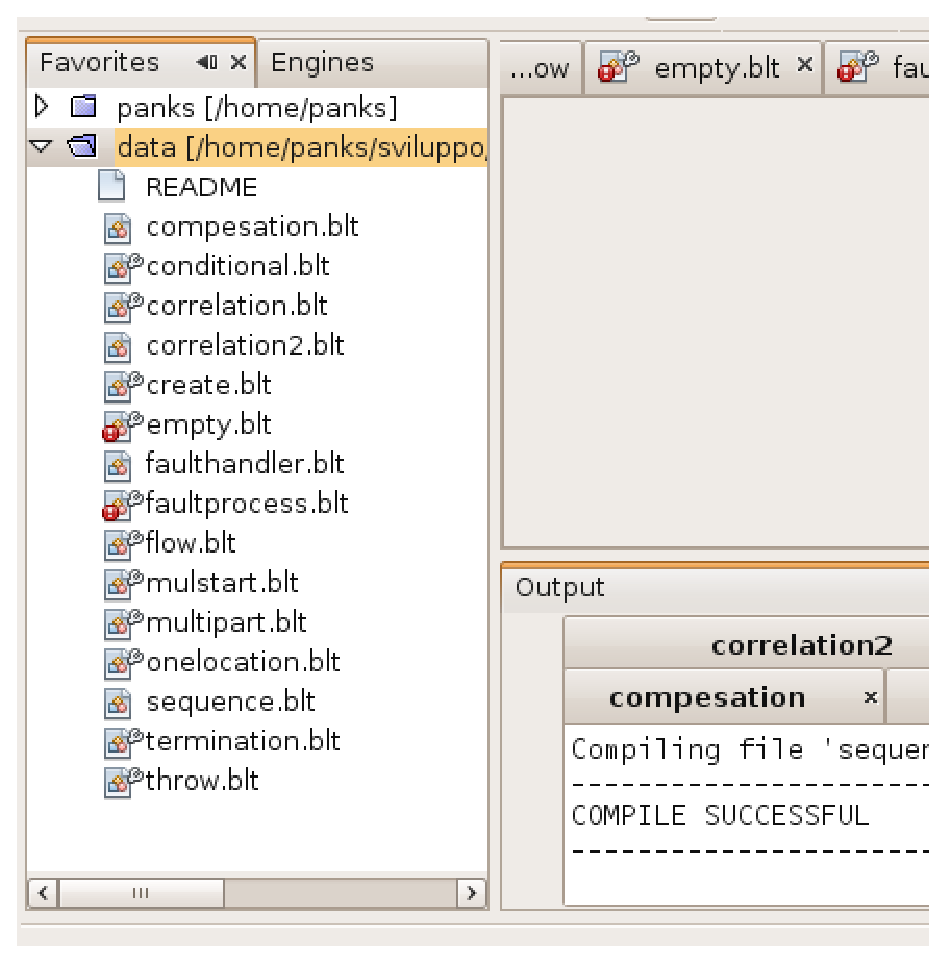
\includegraphics[scale=0.65]
{blide/dia/BlideFavo}
\caption[Il pannello ``Favorites'']{Una direcory con alcuni sorgenti Blite.}
  \label{fig:blideFavo}
\end{center}
\end{figure}

All'interno degli alberi di Favorites i file con estensione
\texttt{.blt} vengono riconosciuti come file sorgenti Blite e vengono
visualizzati con icone speciali. Inoltre l'applicazione decora tali icone in
base al fatto che i file necessitino compilazione, siano stati compilati con
successo o presentino degli errori che ne abbiano compromesso la compilazione.
In Figura \ref{fig:blideFavo} è rappresentato il pannello in cui è stato aggiunto nei
favoriti la directory \texttt{data}, questa contiene una serie di file sorgenti
Blite che vengono visualizzati con le opportune icone. In Tabella
\ref{tab:bicons} sono rappresentate le varie icone associate ai file Blite con il riferimento alla loro semantica.  
\\

\begin{table}
\begin{center}
\begin{tabular}{cp{0.7\textwidth}}

\includegraphics{blide/dia/biconto} & File Blite che deve essere compilato. Il
file non è mai stato compilato o ha subito modifiche dopo l'ultima
compilazione.\\ 
\includegraphics{blide/dia/biconko} & File Blite che presenta
errori di compilazione. L'ultima compilazione eseguita sul file ha riportato errori.\\

\includegraphics{blide/dia/biconok} & File Blite compilato con successo.
Delle definizioni presenti nel file sono disponibili i modelli statici.\\
\end{tabular}
\caption{Icone associate ai file Blite con estensione \texttt{.blt}}
\label{tab:bicons}
\end{center}
\end{table}

Su ogni nodo rappresentante un file Blite possono essere eseguite diverse
azioni. In particolare tali azioni, come è consuetudine nelle applicazioni con
interfaccia grafica, possono essere eseguite in modi diversi: dai menù a
discesa della \emph{``Menu Bar''}, che si trova nella parte alta della finestra,
dai menù contestuali che si aprono premendo il tasto destro del mouse su
un oggetto selezionato e dai bottoni che si trovano nello spazio subito sotto
la menù bar detto \emph{``Tool Bar''}. In Figura \ref{fig:blideCMenu} è rappresentato il
menù contestuale che viene visualizzato premendo il tasto destro su un file
Blite, che nel caso specifico deve essere ancora compilato, per cui risulta
abilitata l'azione \emph{``Compile''}, mentre le azioni \emph{``Re/Deploy''} e
\emph{``Undeploy''} sono ovviamente disabilitate, in quanto non è ancora
disponibile un modello di definizione da poter istallare. In generale
tutta l'interfaccia è stata realizzata secondo il paradigma
\emph{Context-Sensitive Interface} [ContxSensWikiPedia], per cui le sue
varie parti sono sensibili allo stato degli oggetti che si trovano a gestire.

\begin{figure}[t]
\begin{center}
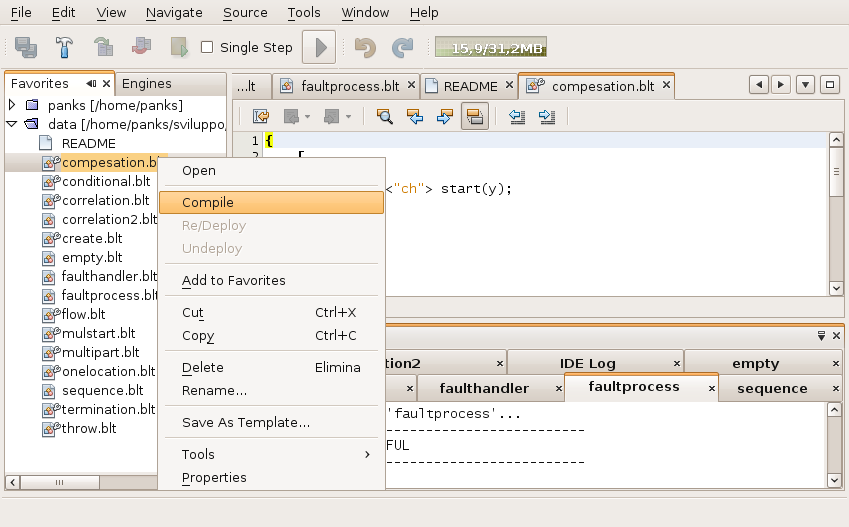
\includegraphics[scale=0.70]
{blide/dia/BlideCMenu}
\caption[Menu Contestuale su di un File Blite]{Facendo click con il tasto destro
su un nodo rappresentante un file Blite, si apre un menù contestuale che
visualizza le azioni che l'utente può compiere sul file stesso. Da osservare
come siano abilitate solo le azioni applicabili, di fatto viene realizzato il
paradigma \emph{Context-Sensitive Interface}, secondo cui ogni componente
dell'interfaccia è sensibile allo stato degli oggetti contestuali.}
  \label{fig:blideCMenu}
\end{center}
\end{figure}

Oltre che nel menù contestuale che si apre sui file Blite, le operazioni che
risultano più frequentemente eseguite dall'utente, \emph{``Save''},
\emph{``Compile''}, \emph{``Deploy''} e \emph{``Undeploy''}, sono state rese
disponibili tramiti pulsanti, facilmente raggiungibili, posizionati nella Tool
Bar:

\begin{center}

\includegraphics[scale=0.70]
{blide/dia/BlideFileToolBar}
\end{center}

Si osservi come anche questa parte dell'interfaccia risulti sensibile al
contesto, cioè in questo caso al file attualmente selezionato o visualizzato
nell'editor, e come siano attivati solamente i pulsanti, le cui azioni siano
attualmente applicabili. 

In Tabella \ref{tab:blideactions} sono ricapitolate le azioni eseguibili su file Blite con le
icone presentate nell'interfaccia.

\begin{table}
\begin{center}
\begin{tabular}{c p{0.7\textwidth} }

\includegraphics[scale=0.8]{blide/dia/build24} & Compilazione del codice
Blite.\\ 

\includegraphics[scale=0.8]{blide/dia/deploy24} & Istallazione dei Deployment
contenuti nel file sugli Engine.\\

\includegraphics[scale=0.8]{blide/dia/undeploy24} & Rimozione dei Deployment
contenuti nel file dagli Engine.
\end{tabular}

\caption{Azioni che possono essere eseguite su un file Blite.}
\label{tab:blideactions}
\end{center}
\end{table}


\newpage

\subsubsection*{Editing e compilazione del codice Blite}
Facendo doppio click, o usando l'azione contestuale \emph{``Open''}, su un nodo
degli alberi di Favorites rappresentate un file Blite, si apre un pannello di
editing nell'opportuna sezione dell'interfaccia grafica. 

Per creare un nuovo file invece si devono eseguire i seguenti passi:

\begin{enumerate}
  \item Nel pannello Favorites, selezionare la directory in cui si desidera
  creare il nuovo file.
  \item Premere il tasto destro e visualizzare il menù contestuale.
  \item Su di questo posizionarsi sulla voce \emph{``New''} in modo da
  visualizzare il sottomenù associato:
\begin{center}
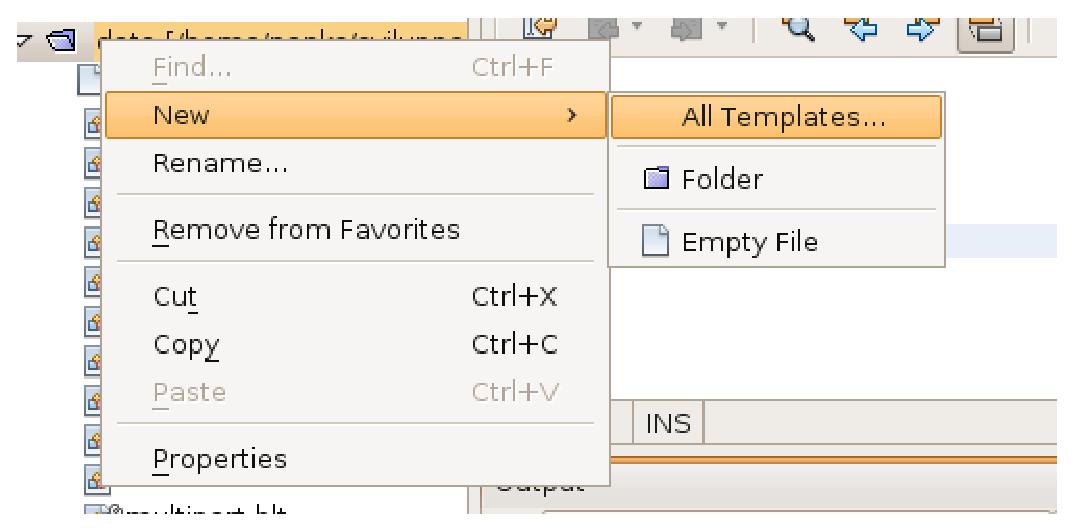
\includegraphics[scale=0.60]{blide/dia/BlideNewFile}
\end{center}
  \item A questo punto le possibilità sono due:
\begin{enumerate}
  \item Creare un file vuoto, selezionando la voce di menù \emph{``Empty
  File''}. In questo caso si aprirà una finestra in cui l'utente potrà digitare
  il nome del nuovo file comprensivo dell'estenzione \texttt{.blt}.
  \item Utilizzare un file di esempio da cui iniziare a
  sviluppare il proprio programma Blite scegliendo la voce \emph{``All
  Templates \ldots''}. In questo caso tramite un ``Wizard'' l'utente potrà
  scegliere fra una serie di file che possono costituire un punto di partenza
  (Template) per scrivere il proprio codice.
\end{enumerate} 
\end{enumerate}

Abbiamo mostrato come aprire un sorgente Blite all'interno di un editor. Blide
fornisce un editor specializzato per scrivere programmi Blite, che mette a
disposizione le funzionalità specifiche di:

\begin{itemize}
  \item \emph{Syntax Highlight}: Tramite la grammatica formale, presentata
  nel Capitolo 2,  è stato possibile realizzare una tecnologia capace di 
  riconoscere la sintassi Blite e evidenziare in maniera opportuna le parole
  riservate  e i costrutti specifici del linguaggio. Tale tecnologia si basa
  sul progetto \emph{``Generic Languages Framework (GLF)''} [GLFSite], che mette
  a disposizione un modulo per NetBeans Platform con cui è possibile sviluppare 
  il supporto ad un linguaggio di programmazione all'interno delle proprie 
  applicazioni.
  
  \item \emph{Autocompletamento}: L'editor dei file Blite assistono
  l'utente nella scrittura del codice andando a completare automaticamente
  alcune parti del codice. In particolare l'editor inserisce automaticamente i
  delimitatori di chiusura dei blocchi. Per esempio all'utente basterà digitare
  la stringa \texttt{seq} e il sistema inserirà automaticamente la chiusura
  inserendo il corrispettivo \texttt{qes}. Inoltre anche le operazioni di
  invocazione e ricezione sono completate automaticamente, digitando per
  esempio semplicemente la stringa \texttt{rcv} l'utente si troverà a
  disposizione l'intera struttura della operazione di ricezione come: 
  \verb#rcv<"on_me"> operation(x)#, e in questa potrà modificare
  le parti necessarie.
  
\end{itemize}

Abbiamo visto come la sintassi originale di Blite sia stata arrichita con
alcune parole riservate e come tutte le attività strutturate siano state
dotate di delimitatori di blocco. Con il supporto dell'editor tale
appesantimento sintattico non verrà avvertito dal programmatore.
  
In Figura \ref{fig:blideEditor} è raffigurato un editor con il sorgente Blite in
cui sono evidenzite tramite colori e font specifici le parole riservate e i costrutti
del linguaggio.
	
La compilazione del file visualizzato nell'editor attualmente attivo, come
detto, può essere eseguita con l'opportuno pulsante nella Tool Bar. All'utente
verrà notificato l'esito della compilazione nell'aria in basso
dell'interfaccia grafica identificata con l'etichetta \emph{``Output''}. In caso di
errore tale area riporterà il messaggio opportuno e l'utente potrà direttamente
fare click su di esso per posizionare automaticamente il cursore dell'editor in
corrispondenza della linea e della colonna in cui è presente l'errore. In
Figura \ref{fig:blideCompError} è rappresentata questa situazione.

\begin{figure}[t]
\begin{center}
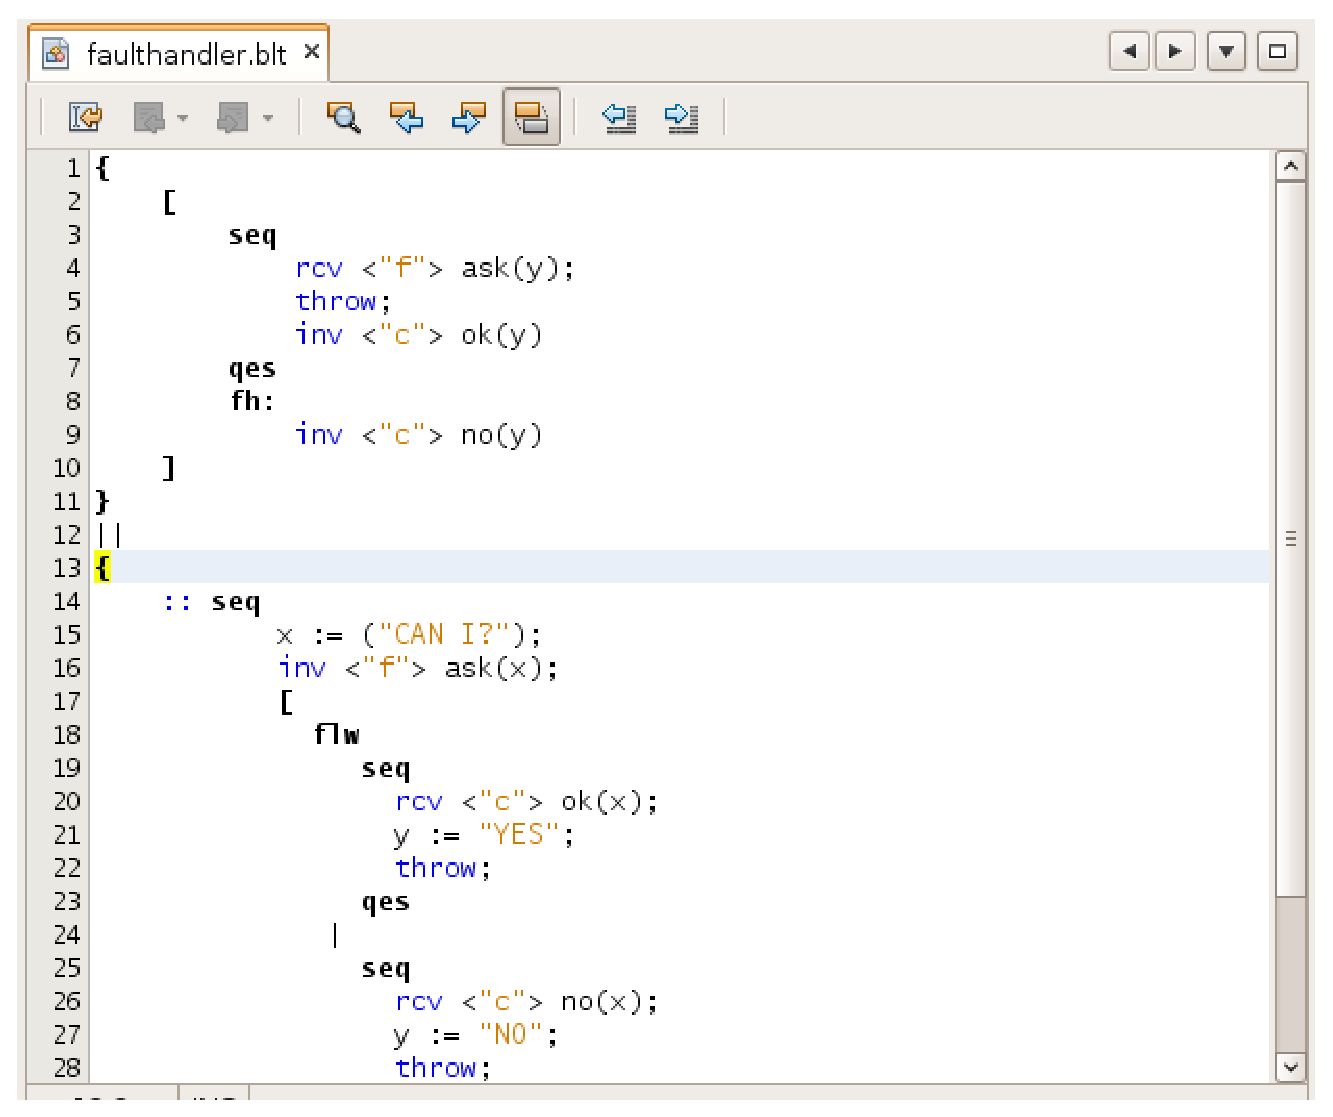
\includegraphics[scale=0.60]
{blide/dia/BlideEditor}
\caption[Blide, l'editor per Blite]{L'edior di Blide per con il \emph{``Syntax
Highlight''} per il codice Blite.}
  \label{fig:blideEditor}
\end{center}
\end{figure}

\begin{figure}[b!]
\begin{center}
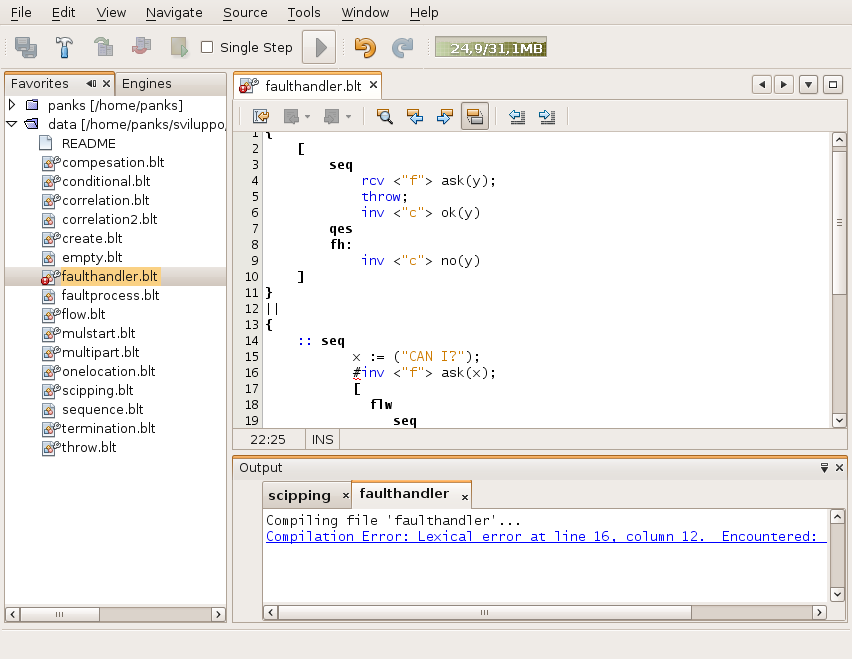
\includegraphics[scale=0.60]
{blide/dia/BlideCompError}
\caption[Blide, feedback alla compilazione]{Feedback interattivo per gli errori
di compilazione.}
  \label{fig:blideCompError}
\end{center}
\end{figure}

\newpage

\subsubsection*{Engines - Deploy ed esecuzione dei processi}

Blide è dotato di un ambiente \emph{Local Environment} per l'esecuzione dei
processi Blite. Come già detto il Local Environment permette di eseguire
localmente (in una Java Virtual Machine) più Engine e di gestire la
comunicazione fra questi simulando la rete.

Quando un file sorgente di Blite è compilato, è abilitata per questo l'azione
di \emph{``Deploy''}; a questo punto se l'utente la esegue i \emph{Deployment}
(si ricorda che nella sintassi i deployment sono individuati dai delimitatori
$\verb#{# \ldots \verb#}#$) definiti nel file e vengono istallati su
opportuni Engine.

Attualmente, per velocizzare il processo di sviluppo dell'utente, l'associazione
Engine-Deployment è fatta in maniera automatica dal tool secondo il seguente
schema:

\begin{itemize}
  \item Ogni Deployment ha il proprio Engine di esecuzione.
  \item L'Engine di un Deployment viene identificato nel seguente modo: 
  
  (``nome file che definisce il deployment'' \texttt{:} ``numero d'ordine del
  dep. nel file'')
  
  Per cui, se abbiamo che un deployment è il terzo definito nel file
  \texttt{source.blt} esso verrà istallato in un engine identificato con
  l'etichetta: \texttt{source.blt:3}.
\end{itemize}

Nell'interfaccia, il pannello identificato con l'etichetta \emph{``Engines''}
visualizza un albero, la cui radice è contrassegnata come \emph{``Local
Engines''}. I nodi figli della radice rappresentano gli Engine attualmente
presenti nel Local Environment identificati con la convenzione sopra esposta;
espandendo i loro figli troviamo le definizioni di processo, e per ognuna di
essa, a livello inferiore troviamo le istanze.

\begin{figure}[t]
\begin{center}
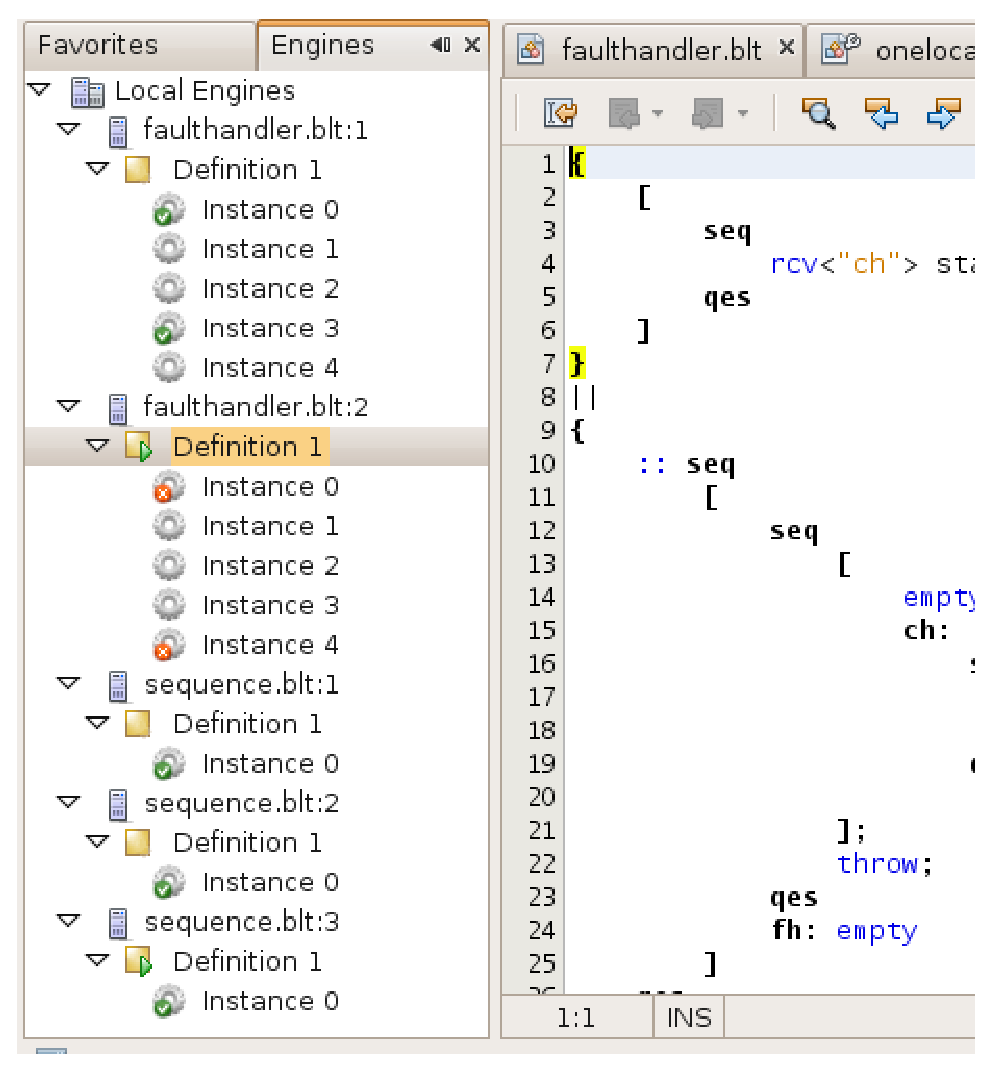
\includegraphics[scale=0.65]
{blide/dia/BlideEngines}
\caption[Blide, feedback alla compilazione]{Rappresentazione del Local
Environment con gli Engine, in questi le definizioni di processo istallate. Per
ogni definizione sono visualizzate le istanze eseguite o in esecuzione.}
  \label{fig:blidEngines}
\end{center}
\end{figure}

In Figura \ref{fig:blidEngines} è presentato l'albero dei Local Engines.
Come si può osservare fra le definizioni istallate negli Engine, si può
distinguere le così dette \emph{Ready to Run Instancess}, da queste l'utente
può avviare direttamente delle istanze tramite l'operazione contestuale
\emph{``Run''}, o tramite l'opportuno pulsante posizionato nella Tool Bar.

\begin{center}
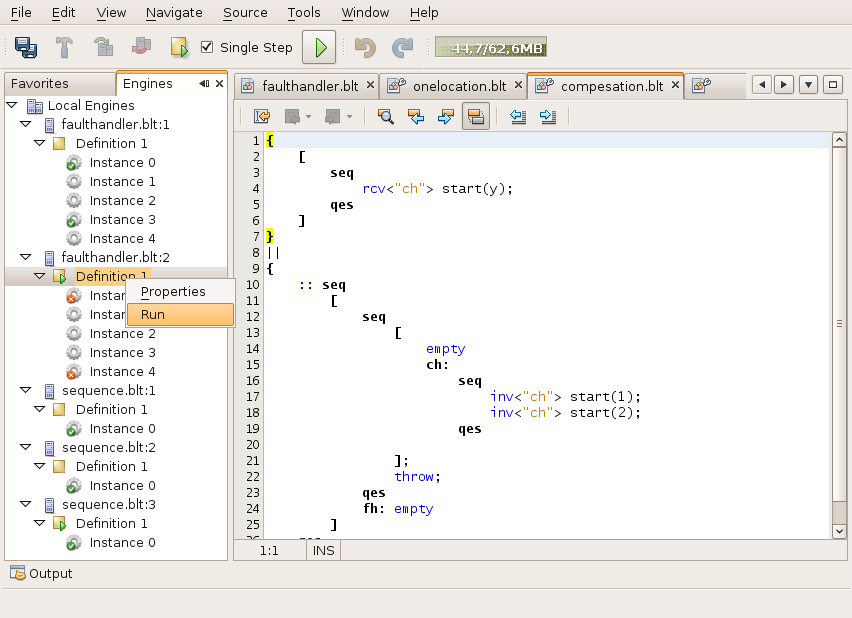
\includegraphics[scale=0.65]{blide/dia/BlideRunInst}
\end{center}

In tabella sono riepilogati (con le rispettive Icone) i vari tipi di nodi che
si trovano nei livelli dell'albero dei Local Engines.

\begin{table}[hb!]
\begin{center}
\begin{tabular}{rp{0.7\textwidth}}

\includegraphics[scale=0.70]{blide/dia/server} & Engine.\\ 

\includegraphics[scale=0.70]{blide/dia/defnode} & Definizione di Processo.\\

\includegraphics[scale=0.70]{blide/dia/defnodeRun} & Ready to Run Instance.\\

\includegraphics[scale=0.70]{blide/dia/instdef} & Istanza in esecuzione.\\

\includegraphics[scale=0.70]{blide/dia/instdefok} & Istanza completata.\\

\includegraphics[scale=0.70]{blide/dia/instdefko} & Instanza terminata con
errori .\\
\end{tabular}
\caption{I vari tipi di nodi nell'albero Local Engines.}
\label{tab:bicons}
\end{center}
\end{table}

\newpage

\subsubsection*{Monitor - Visualizzazione dell'istanze}

Abbiamo visto come l'utente possa scrivere i propri programmi Blite, istallarli
ed eseguirli all'interno di un Local Environment. L'esecuzione viene avviata
facendo partire una definizione di tipo \emph{Ready to Run Instance}, da
questa verrà creata immediatamente un'istanza che probabilmente, invocando le
porte di start activity di altre definizioni di processo, provocherà la
creazione di altre istanze. Per esempio si consideri il caso

\vspace{0.5cm}
\begin{center}
\begin{tabular}{ccc}
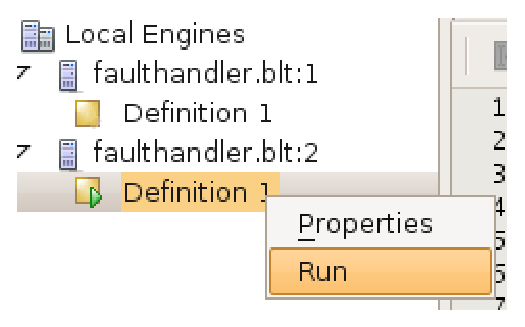
\includegraphics[scale=0.75]{blide/dia/BlideMon1} 
& $\Rightarrow$
& 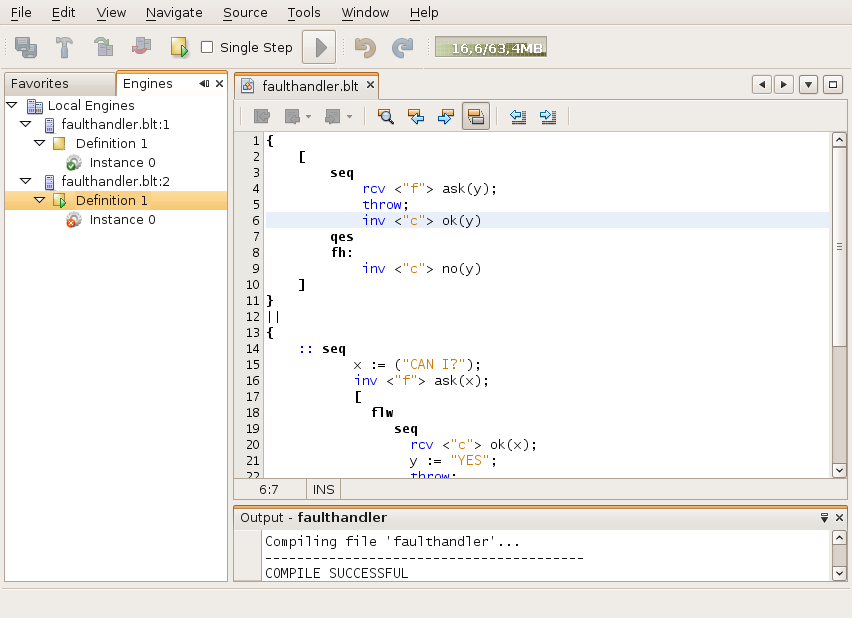
\includegraphics[scale=0.75]{blide/dia/BlideMon2}    
\end{tabular}
\end{center}
\vspace{0.5cm}

in cui si hanno due Engine: \texttt{faulthandler.blt:1} con la definizione
\texttt{Definition 1} e \texttt{faulthandler.blt:1} con la \emph{Ready to Run
Instance} \texttt{Definition 1}. Quest'ultima può essere messa in esecuzione
direttamente dall'utente facendo click con il tasto destro e selezionando dal
menù contestuale l'azione \emph{``Run''}. A questo punto come si vede dalla
figura a destra vengono generate due istanze; la Ready to Run Instance ha
provocato la creazione di un'istanza della definizione di processo istallata su
\texttt{faulthandler.blt:1}.

Già dalla rappresentazione delle istanze nell'albero Local Engines si ha una
informazione sull'esito della loro esecuzione. Come precedentemente detto
le icone riportano graficamente il fatto che un'istanza abbia concluso con
esito positivo o meno la propria elaborazione. 

All'utente viene data inoltre, la possibilità di visualizzare il flusso
completo di esecuzione di un'istanza. Facendo doppio click sul nodo
dell'istanza si apre, nella zona dedicata agli editor, un pannello
che propone una rappresentazione grafica dell'esecuzione della stessa. Tale
pannello viene di seguito identificato con il termine \emph{Monitor View}.

\begin{figure}[p]
\begin{center}
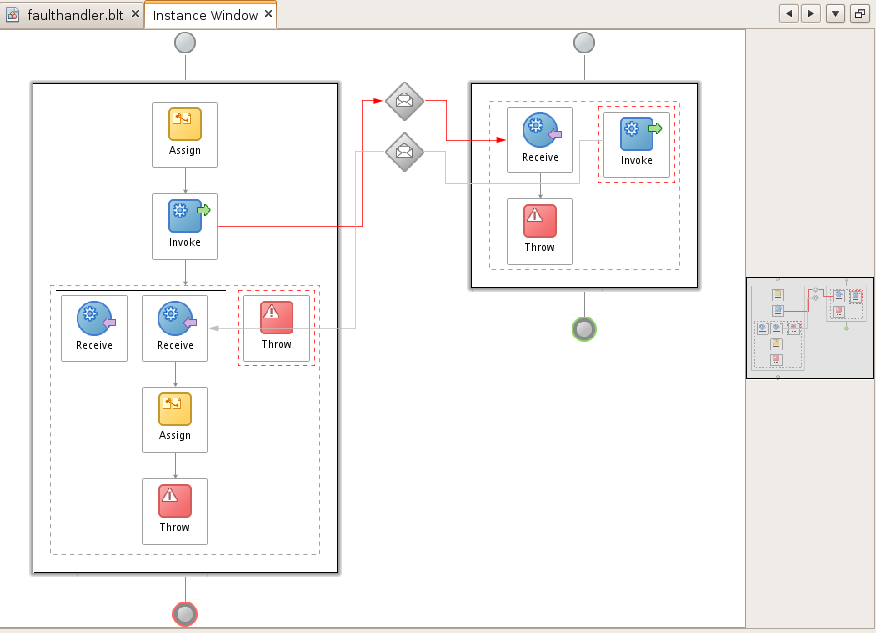
\includegraphics[scale=0.65,angle=90]
{blide/dia/BlideMonitor1}
\caption[]{}
  \label{fig:blideMonitor1}
\end{center}
\end{figure}

\begin{figure}[!t]
\begin{center}
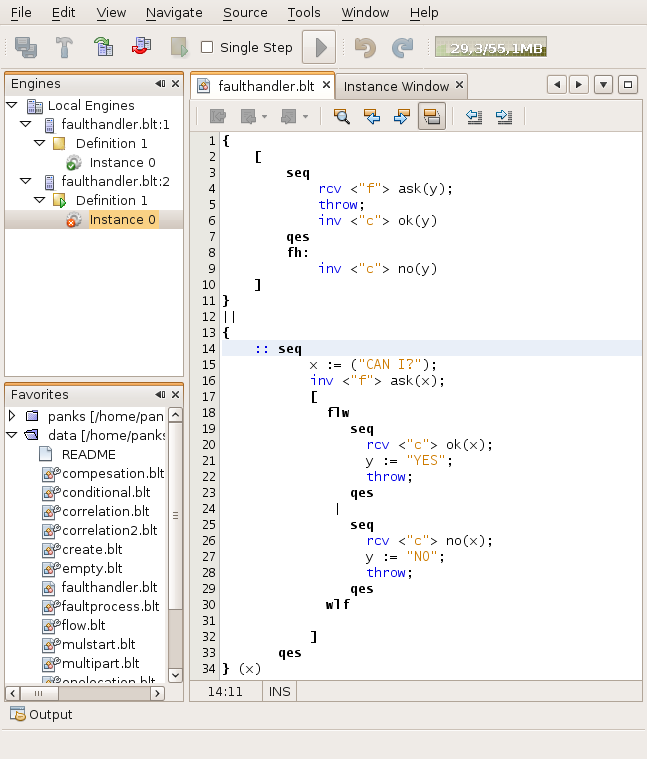
\includegraphics[scale=0.79]
{blide/dia/BlideMonitorCode}
\caption[]{}
  \label{fig:blideMonitorCode}
\end{center}
\end{figure}


Disponendo già di un Monitor View aperto, l'utente vi può aggiungere altre
istanze trascinandocele sopra, secondo il paradigma \emph{Drag-and-Drop}. In
questo modo è possibile visualizzare in un'unica rappresentazione grafica
l'interazione di più istanze di processo che nel loro ciclo di vita si sono
scambiate messaggi. In Figura \ref{fig:blideMonitor1} è rappresentato il
Monitor View con la rappresentazione dell'esecuzione di due istanze generate
dal codice di Figura \ref{fig:blideMonitorCode}. Si noti come la Ready to Run
Instance tramite la prima invocazione produca la creazione dell'istanza
derivante dalla definizione di processo, quest'ultima con una successiva
invocazione risponde con un messaggio di correlazione. Si osservi inoltre come
l'istanza di destra concluda con successo la sua esecuzione, in quanto
l'eccezione sollevata è gestita in un Fault Handler (è il Fault Handler stesso
che esegue l'invocazione di risposta). Quella di sinistra invece fallisce poiché
l'eccezione sollevata non è gestita da alcun Fault Handler e la stessa produce
la terminazione del ramo parallelo che era fermo in attesa di ricevere un
messaggio. 

A prima vista potrebbe sorpredere la presenza della seconda Throw (racchiusa
dal rettangolo tratteggiato di rosso) nell'istanza fallita, in quanto non
sembrerebbe prevista dal codice. In realtà essa non è altro che l'attività
Throw prevista dal Default Fault Handler (si veda \ref{defHandelr}). C'e'
sembrato che la scelta migliore per rendere la rappresentazione grafica più chiara possibile fosse
quella di rappresentare esplicitamente i Default Fault Handler, in quanto
condizionano fortemente il flusso di esecuzione, e di nascondere al contrario i
Default Compensation Handler (Empty Activity) in quanto del tutto ininfluenti.
\\

Concludiamo questa sezione dando una panoramica dei costrutti grafici utilizzati
per rappresentare i flussi di esecuzione.
\vspace{0.3cm}

\begin{tabular}{cp{0.6 \textwidth}}
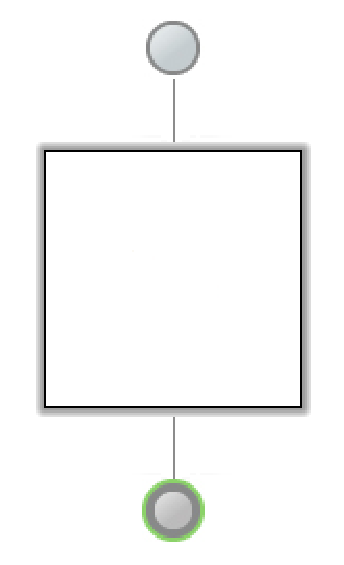
\includegraphics[scale=0.48]{blide/dia/BlideInst} &
\parbox[b][4cm][t]{0.6 \textwidth}{Le istanze di processo
sono rappresentate tramite scatole (ombreggiate) che contengono le attvità.
Le scatole presentano alle estremità due cerchi, di cui quello in basso,
tramite la sua colorazione indica lo stato della richiesta: grigio, in
esecuzione, verde completata con successo, rosso fallita.}
\\
\end{tabular}

\begin{tabular}{cp{0.6 \textwidth}}

\includegraphics[scale=0.80]{blide/dia/BlideInv} &
\parbox[b][2.5cm][t]{0.6 \textwidth}{Le attività di base (\emph{Basic
Activity}), sono rappresentate come dei quadrati con all'interno una opportuna
icona la cui grafica rimanda alla semantica della attività.}
\end{tabular}

\begin{tabular}{cp{0.6 \textwidth}}

\includegraphics[scale=0.95]{blide/dia/BlideSec} &
\parbox[b][1.7cm][t]{0.6 \textwidth}{L'attività di sequenza è rappresentata con
una freccia verticale, che unisce dall'alto verso il basso le attività
sequenzializzate. Le attività che cronologicamente sono eseguite prima si
trovano più in alto.}
\end{tabular}

\vspace{0.5cm}

\begin{tabular}{cp{0.6 \textwidth}}
\parbox[b][1.2cm][t]{0.17 \textwidth}{

\includegraphics[scale=0.40]{blide/dia/BlideFlow}} 
&
\parbox[b][1.7cm][t]{0.6 \textwidth}{L'attività di composizione parallela è
rappresentata come una barra orizzontale sotto di cui, da sinistra a destra,
vengono rappresentati i flussi di esecuzione.}
\end{tabular}


\begin{tabular}{cp{0.6 \textwidth}}

\includegraphics[scale=0.30]{blide/dia/BlideContext} & 
\parbox[b][2.2cm][t]{0.6 \textwidth}{I contesti sono rappresentati come
rettangoli tratteggiati, al cui interno viene svolta la Context Activity. Se il
contesto attiva un Protected Scope, questo viene rappresentato a partire
dell'angolo in alto a destra come un rettangolo con il bordo tratteggiato di
colore rosso.}
\end{tabular}

\vspace{1.5cm} 

\begin{tabular}{cp{0.6 \textwidth}}
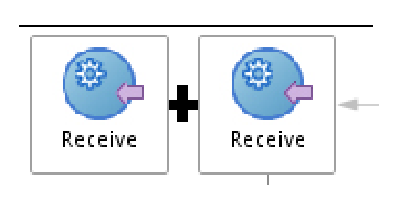
\includegraphics[scale=0.42]{blide/dia/BlidePick} & 
\parbox[b][1.5cm][t]{0.6 \textwidth}{La scelta esterna è rappresentata tramite
la disposizione orizzontale delle attività di ricezione unite dal simbolo +.}
\end{tabular}

% \caption{tablecaption}
% \label{tablelabel}
% \end{table}

\section{Un esempio d'uso}